\documentclass[10pt]{beamer}
%\documentclass[handout,10pt]{beamer}
%\mode<presentation>
%{
%  \usetheme{Berkeley}
%  \usecolortheme{seahorse}
%  \usefonttheme{default}
%  \setbeamertemplate{navigation symbols}{}
%  \setbeamertemplate{caption}[numbered]
%}

\usetheme{metropolis}

\usepackage[english]{babel}
\usepackage[utf8x]{inputenc}
\usepackage{caption}
\usepackage{multirow}
\usepackage{mathrsfs}
\usepackage{graphicx}
\usepackage{amsmath}
\usepackage{graphicx}
\usepackage[compatibility=false]{caption}
\usepackage{subcaption}
\usepackage[normalem]{ulem}
\DeclareMathOperator{\tr}{tr}
\usepackage{textpos}
\usepackage{animate}

\title[FMSP Further Mathematics]{Trigonometry, Sets \& Functions}
%\titlegraphic{\includegraphics[height=1.57cm]{logo.jpg}}
\author[Scott Morgan]{\textbf{Scott Morgan}}
\institute{\textit{Further Mathematics Support Programme - WJEC A-Level Further Mathematics} \\
\textit{17th February 2018}
\\ \\ \\
\textit{scott3142.com | @Scott3142}}
\date

\begin{document}

\begin{frame}
  \maketitle
\end{frame}

\begin{frame}{Trigonometry, Sets \& Functions}
	\begin{enumerate}
		\item [1.] Sets \& Functions
	\end{enumerate}
\end{frame}

\begin{frame}{Properties of Real Functions}
  \begin{itemize}[<+->]
    \item Even/Odd/Neither
    \item Continuous/Discontinuous
    \item Increasing/Decreasing/Neither
    \item Bounded/Unbounded
  \end{itemize}
\end{frame}

\begin{frame}{Real Functions - Even \& Odd}
  \begin{itemize}[<+->]
  	\item A function is \textbf{even} if its graph has the $y$ axis as a line of symmetry.
  	\begin{itemize}
  		\item For an even function, $f(-x) = f(x)$
  	\end{itemize}
  	\item A function is \textbf{odd} if its graph has \textit{rotational symmetry of order 2} about the origin.
  	\begin{itemize}
  		\item For an odd function, $f(-x) = -f(x)$
  	\end{itemize}
	\item A function can be \textit{neither} even \textit{nor} odd.
	\item Can you think of any examples?
  \end{itemize}
\end{frame}

\begin{frame}{June 2008 - Q1}
  \begin{itemize}[<+->]
    \item For each of the following functions state, with a reason, whether it is \textit{even}, \textit{odd} or \textit{neither even nor odd}.
    \begin{enumerate}
    	\item <2-3> $\frac{x}{x^2+1}$
    	\item <4-> $e^x + 1$
    \end{enumerate}
  \end{itemize}

  \only<3>{
  	\begin{itemize}
	  	\item $f(-x) = \frac{-x}{(-x^2)+1} = -\left(\frac{x}{x^2+1}\right) = -f(x)$
	  	\item Hence, the function is odd. 
	\end{itemize}
  }

	\only<5>{
		\begin{itemize}
			\item $f(-x) = e^{-x} + 1$  which is neither $f(x)$ or $-f(x)$.
			\item Hence, the function is neither even nor odd. 
		\end{itemize}
	}
\end{frame}

\begin{frame}{Continuous \& Discontinuous}
  \begin{itemize}[<+->]
  	\item A function $f(x)$ is called continuous if the graph of the function consists of a single unbroken line.
  	\item <2> The function $f(x) = \frac{x+1}{x-1}$ has a discontinuity at $x=1$.
  	\item <3> Consider the function $f(x) = \begin{cases} x^2 - 2x + 4, & x > 2 \\ -x^2 + 6x - 7, & x \leq 2 \end{cases}$ 
  \end{itemize}

  \only<2>{
	\begin{figure}
		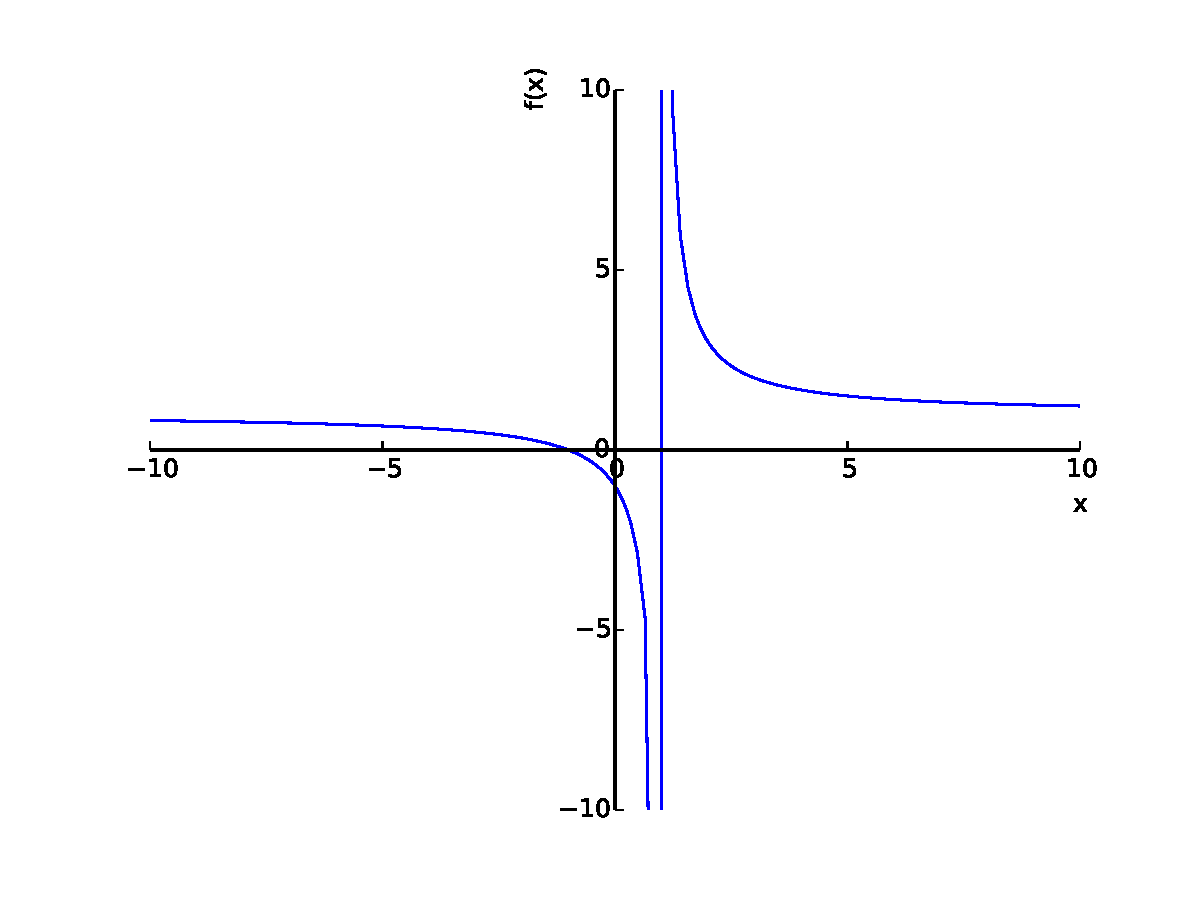
\includegraphics[width=\textwidth]{beamer-pics/continuous-1.pdf}
		\caption{Functions that are algebraic fractions are discontinuous when the denominator is zero.}
	\end{figure}
  }

  \only<3>{
	\begin{figure}[t!]
		\centering
		\begin{subfigure}[b]{0.49\textwidth}
			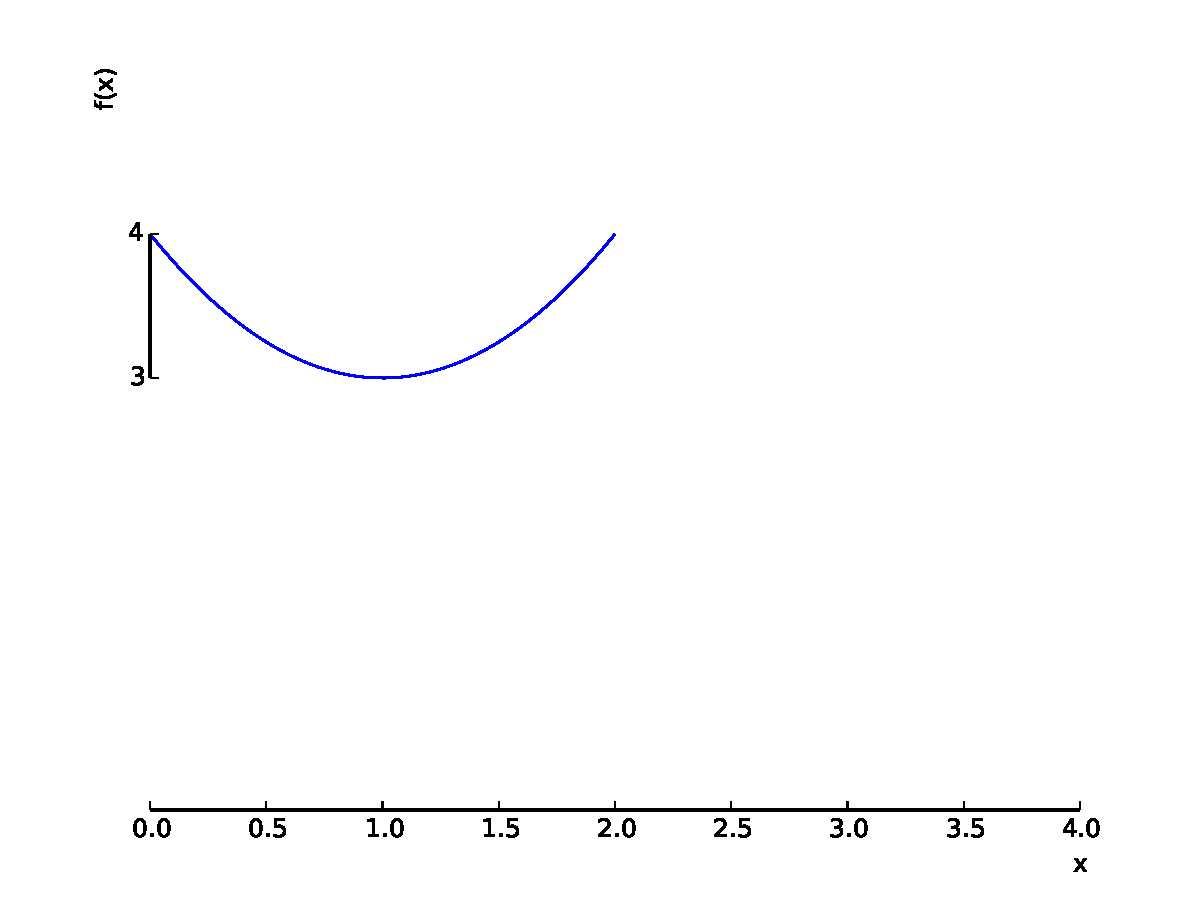
\includegraphics[scale=0.11]{beamer-pics/continuous-2.pdf}
			\caption*{}
		\end{subfigure}	
		\begin{subfigure}[b]{0.49\textwidth}
			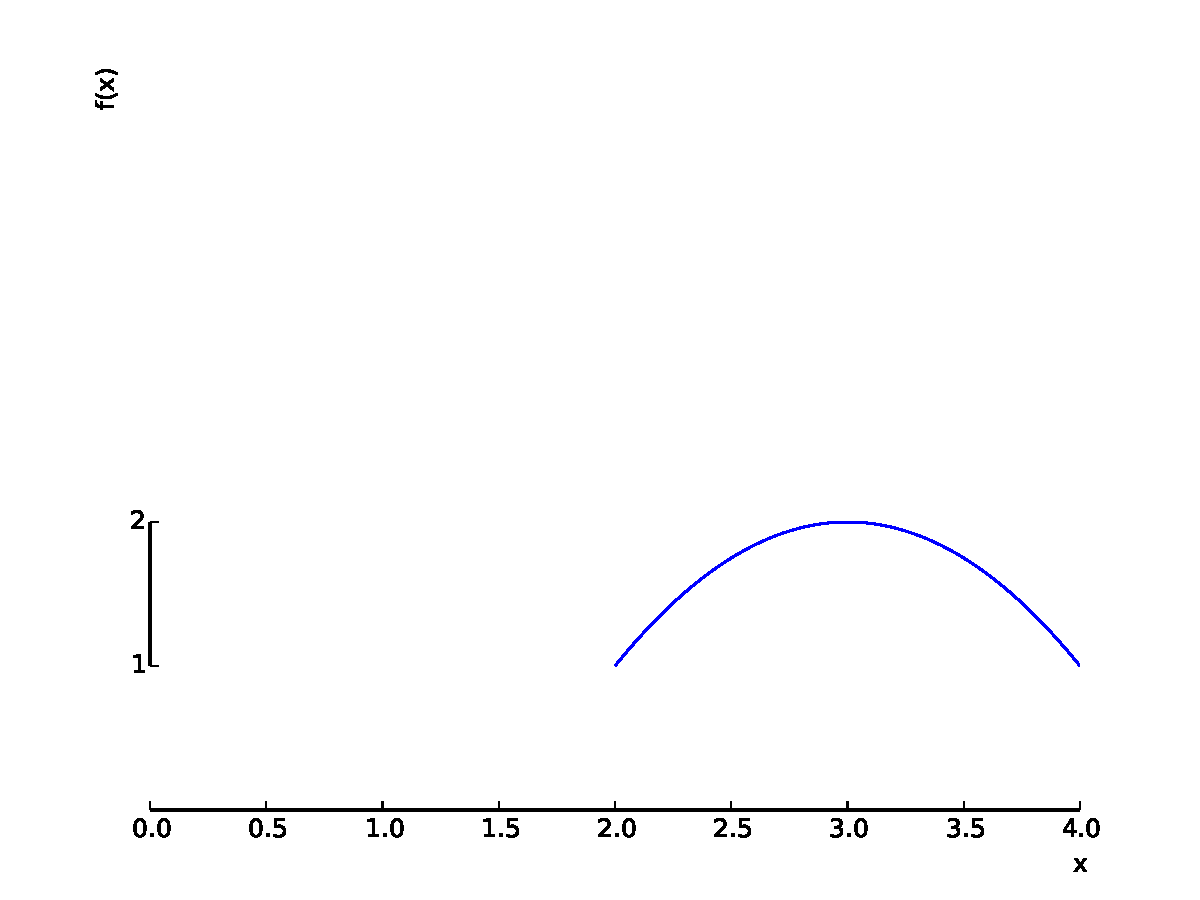
\includegraphics[scale=0.11]{beamer-pics/continuous-3.pdf}
			\caption*{}
		\end{subfigure}
		\caption{This function is made from two functions and has a jump at $x=1$.}
	\end{figure}
  }
\end{frame}

\begin{frame}{Real Functions - Increasing/Decreasing}
	\only<1-3>{
	  \begin{itemize}[<+->]
		\item <1-3> A function $f(x)$ is called \textbf{strictly decreasing} if the value of $f(x)$ decreases as $x$ increases.
		\item <2-3> This means that the gradient of the functions is negative (not including zero) for all values of $x$.
	\end{itemize}
}

	\only<4-6> {
	\begin{itemize}
		\item <4-6> A function $f(x)$ is called \textbf{strictly increasing} if the value of $f(x)$ increases as $x$ increases.
		\item <6> This means that the gradient of the functions is positive (not including zero) for all values of $x$.
	  \end{itemize}
  }

  \only<3>{
	\begin{figure}
		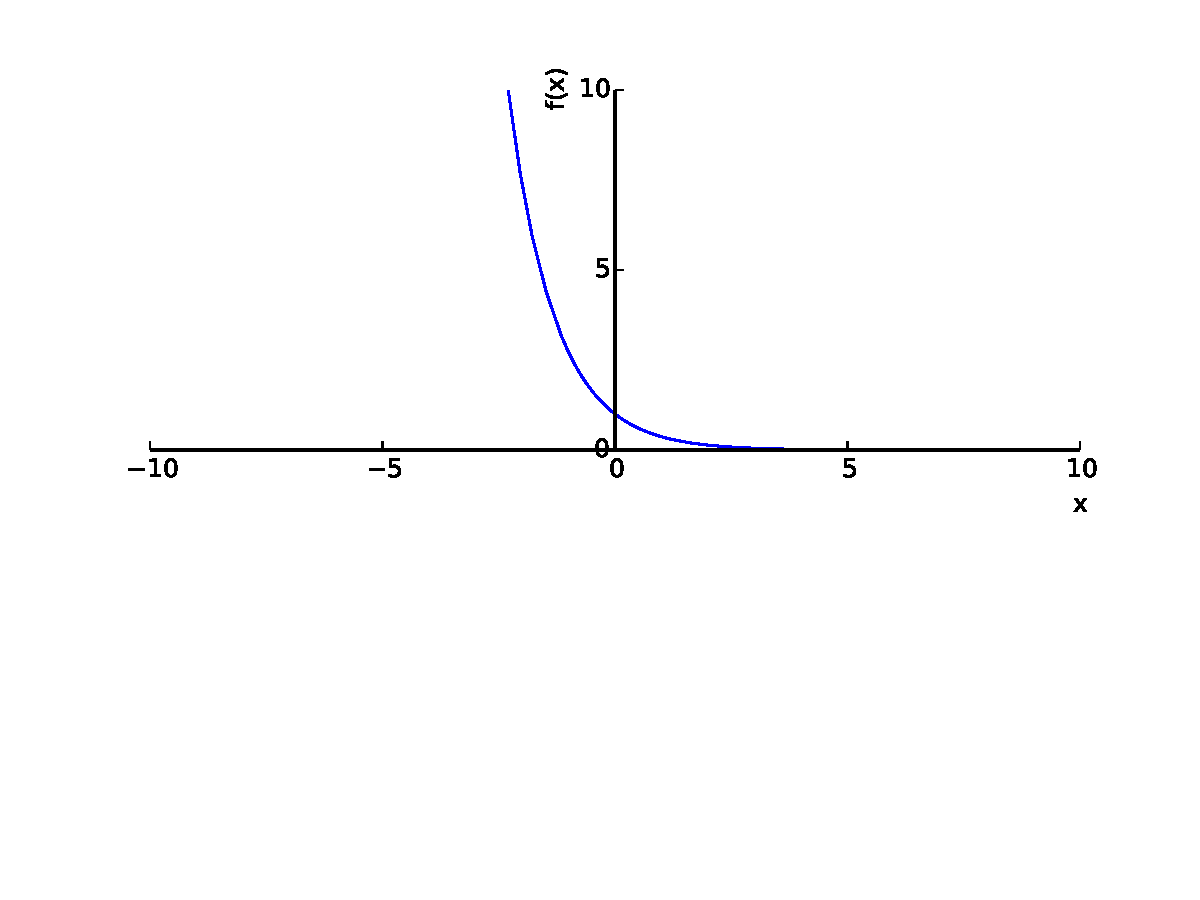
\includegraphics[width=\textwidth]{beamer-pics/decreasing.pdf}
	\end{figure}

	\begin{itemize}
		\item The function $f(x) = e^{-x}$ is strictly decreasing. The gradient function is given by $f'(x) = -e^{-x}$, which is negative for all values of $x$.
	\end{itemize}
  }

  \only<6>{
	\begin{figure}
		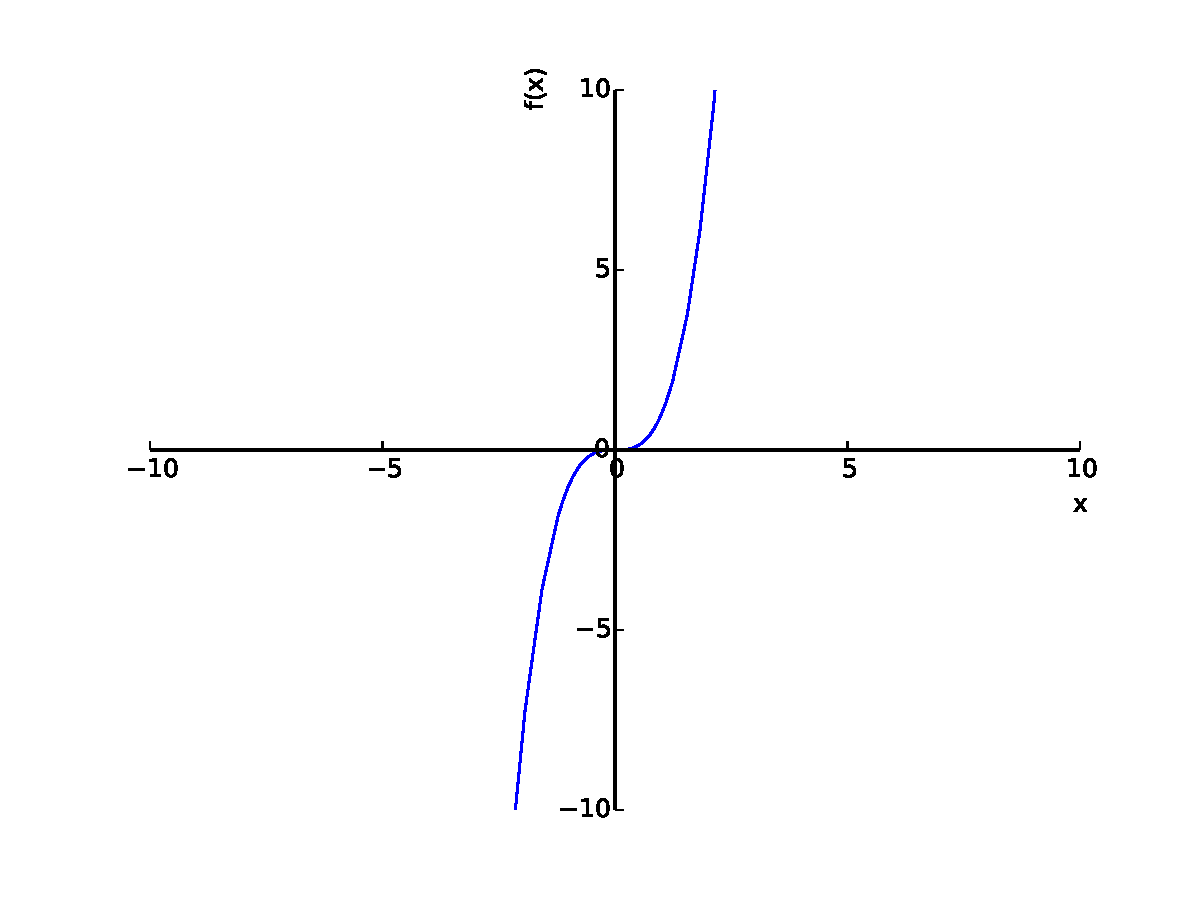
\includegraphics[width=\textwidth]{beamer-pics/increasing.pdf}
	\end{figure}

	\begin{itemize}
		\item The function $f(x) = x^3+x+1$ is strictly increasing. The gradient function is given by $f'(x) = 3x^2+1$, which is positive for all values of $x$.
	\end{itemize}
  }

  \only <7-> {
    \begin{itemize}
    	\item  Differentiating a function is often a good way to test these properties.
    \end{itemize}
  }
\end{frame}

\begin{frame}{June 2007 - Q8}
    \begin{itemize}
    	\item The function $f$ is defined on the domain $(0,2)$ by 
    	$f(x) = \begin{cases} 4x^2, & 0 < x < 1 \\ (x+1)^2, &  1\leq x < 2 \end{cases}$ 
    	\begin{enumerate}
    		\item Determine whether or not $f$ is continuous when $x = 1$.
    		\item Show that $f$ is a strictly increasing function.
    		\item Obtain an expression for $f^{-1}(x)$ on each part of its domain.
    	\end{enumerate}
   	\end{itemize}
\end{frame}

\begin{frame}{June 2011 - Q3}
	\begin{itemize}
		\item The piecewise function $f$ is defined by 
		$f(x) = \begin{cases} -x^2 + 6x - 7, & x \leq 2 \\ x^2 - 2x + 4, &  x > 2 \end{cases}$ 
		\begin{enumerate}
			\item Determine whether or not $f$ is continuous for all values of $x$.
			\item Determine whether or not $f$ is a strictly increasing function.
			\item The interval $[1,3]$ is denoted by $A$. Determine $f(A)$.
		\end{enumerate}
	\end{itemize}
\end{frame}

\begin{frame}{Trigonometry, Sets \& Functions}
	\begin{enumerate}
		\item [2.] Trigonometry
	\end{enumerate}
\end{frame}

\begin{frame}{Trigonometric Equations}
	\begin{itemize}[<+->]
		\item A trigonometric equation can have infinitely many solutions. 
		\item We can use the \textbf{general solution formulae} to find them all.
		\item Let $p$ denote the \textit{principle value} of the relevant trig inverse function at point $A$.
	\end{itemize}

	\only<4->{
		\begin{equation*}
			\sin(\theta) = A \only<5->{\implies \theta = n\pi + (-1)^n p, \hspace{3mm} \text{for any integer $n$}}
		\end{equation*}
	}

	\only<6->{
		\begin{equation*}
		\cos(\theta) = A \only<7->{\implies \theta = 2n\pi + p, \hspace{3mm} \theta = (2n-1)\pi - p, \hspace{3mm} \text{for any integer $n$}}
		\end{equation*}
	}

	\only<8->{
		\begin{equation*}
		\tan(\theta) = A \only<9->{\implies \theta = \pm p + 2n\pi, \hspace{3mm} \text{for any integer $n$}}
		\end{equation*}
	}
\end{frame}

\begin{frame}{Examples}
	\begin{itemize}
		\item Find the general solution, in degrees, to each of the following questions:
		\begin{enumerate}
			\item $\sin(x) = 0.3$
			\item $\tan(x) = 1.5$
			\item $\cos(x) = -0.7$
			\item $\sin(x) = -0.6$
		\end{enumerate}
	\end{itemize}
\end{frame}

\begin{frame}{Important Formulae}
	\begin{itemize}
		\item These are in your formula booklet:
		\begin{enumerate}
			\item \textit{Little-$t$} formula:
				\begin{itemize}
					\item <2-> $t = \tan\left(\frac12\theta\right)$
					\item <3-> $\sin(\theta) = \frac{2t}{1+t^2}$
					\item <4-> $\cos(\theta) = \frac{1-t^2}{1+t^2}$
				\end{itemize}
			\item <5-> \textit{Half-angle} formula:
				\begin{itemize}
					\item <6-> $\sin(\alpha) + \sin(\beta) = 2\sin\left[\frac12(\alpha+\beta)\right]\cos\left[\frac12(\alpha-\beta)\right]$
					\item <7-> $\sin(\alpha) - \sin(\beta) = 2\sin\left[\frac12(\alpha-\beta)\right]\cos\left[\frac12(\alpha+\beta)\right]$
					\item <8-> $\cos(\alpha) + \cos(\beta) = 2\cos\left[\frac12(\alpha+\beta)\right]\cos\left[\frac12(\alpha-\beta)\right]$
					\item <9-> $\cos(\alpha) - \cos(\beta) = 2\sin\left[\frac12(\alpha+\beta)\right]\sin\left[\frac12(\alpha-\beta)\right]$
				\end{itemize}
		\end{enumerate}
	\end{itemize}
\end{frame}

\begin{frame}{Important Formulae - When to Use Them:}
	\begin{itemize}
		\item Use the \textit{little-$t$} formula when you are solving an equation with \textit{both} $\cos$ and $\sin$:
			\begin{equation*}
				a\sin(\theta) + b\cos(\theta) = c
			\end{equation*}
		\item <2-> Use the \textit{half-angle} formula when you have \textit{only} $\cos$ or $\sin$:
			\begin{align*}
			\sin(a\theta) + \sin(b\theta) &= c \\
			\cos(a\theta) + \cos(b\theta) &= c
			\end{align*}
	\end{itemize}
\end{frame}

\begin{frame}{June 2006 - Q5}
	\begin{itemize}
		\item By putting $t = \tan\left(\frac{\theta}{2}\right)$, find the general solution of the equation:
		\begin{enumerate}
			\item $3\cos(\theta) + 4\sin(\theta) = 3 - \tan\left(\frac{\theta}{2}\right)$
		\end{enumerate}
	\end{itemize}
\end{frame}

\begin{frame}{June 2009 - Q4}
	\begin{itemize}
		\item Find the general solution to the equation:
		\begin{enumerate}
			\item $\sin(\theta) + \sin(2\theta) + \sin(3\theta) = 0$
		\end{enumerate}
	\end{itemize}
\end{frame}

\end{document}
